\documentclass[a4paper]{article}

\usepackage[portuguese]{babel}
\usepackage[utf8]{inputenc}
\usepackage{amsmath}
\usepackage{graphicx}
\usepackage[colorinlistoftodos]{todonotes}
\usepackage{float}

\title{Relatório Projeto Metódos Numéricos - Parte 1}

\author{
Autor: Thiago Augusto dos Santos Martins - tasm2@cin.ufpe.br
\and
Monitor Chefe: Victor Crisóstomo Mellia - vcm@cin.ufpe.br
\and
Professor: 	Ricardo Martins de Abreu Silva - rmas@cin.ufpe.br
\and
Disciplina: Métodos Numéricos Computacionais - IF816
\and
Período: 2018.2
}

\date{\today}

\begin{document}
\maketitle

\begin{abstract}
Este relatório tem como objetivo analisar os métodos numéricos discutidos em sala de aula e implementados em um programa python. Além de calcular os pontos retornados por cada um desses, explictando as informações das implementações requisitadas e uma análise qualitativa entre os métodos e os valores retornados em si. Para executar o projeto ler o arquivo \textit{README.md}.
\end{abstract}

\section{Métodos Numéricos}
\label{sec:introduction}
Do mesmo modo que temos uma sequência de passos para resolver um sistema de equações linear, como:
$$\begin{cases} 
3x + 5y + z = 3 \\ 7x – 2y + 4z = 2 \\ -6x + 3y + 2z = 0 
\end{cases}$$
também temos uma sequência de passos para solucionar equações diferenciais ordinárias, EDO. 

\begin{equation}
y'(t) = f(t, y(t))
\end{equation}
\centerline{Eq. 1: Exemplo de uma EDO do primeiro grau}
\smallskip\par

Existem passos diferentes para achar a solução de cada tipo de EDO. Que pode depender da sua linearidade, do seu grau, se ela é implícita ou explícita, homogênea ou não. A solução para uma EDO é uma função $y(t)$ cujas derivadas satisfazem a equação, podendo ter mais de uma solução. Se for definido um problema de valor inicial(PVI), teremos uma única solução para a EDO. \par
Mas existem procedimentos numéricos que permitem estimar o valor de pontos da solução dessas EDOs.
Nas próximas secções vamos analisar os metódos de,

\begin{center}
    \begin{minipage}{.4\textwidth}
        \begin{enumerate} 
            \item Euler 
            \item Euler Inverso 
            \item Euler Aprimorado 
            \item Runge-Kutta 
            \item Adam-Bashforth 
            \item Adam-Multon
            \item Fórmula Inversa
        \end{enumerate}
    \end{minipage}
\end{center}
como eles são calculados, exemplos de entrada e saída dos métodos e uma comparação entre eles.

\subsection{Implementação}
Para calcular os métodos foi utilizado a linguagem de programação Python e a biblioteca de matemática simbólica, sympy, que permite um fácil entendimento e resolução de problemas de álgebra computacional.

\section{Análise dos Métodos}
Para as análises do próximos métodos, levaremos em consideração a equação 2 escrita no modelo da equação 1.

\begin{equation}
y'(t) = 1 - t + 4y(t)
\end{equation}
\centerline{Eq. 2: Exemplo de EDO para cálculo das instâncias dos métodos numéricos.}\par

que tem como solução:
\par
\begin{equation}
   y(t) = c_1e^{4t} + \frac{t}{4} - \frac{3}{16} 
\end{equation}
\centerline{Eq. 3: Solução da equação 2.}
\smallskip\par
e para um PVI de $y(0) = 0$, a equação 3 torna-se:

\begin{equation}
  y(t) = \frac{3}{16}e^{4t} + \frac{t}{4} - \frac{3}{16}  
\end{equation}
\centerline{Eq. 4: Solução da equação 2 para o PVI: $y(0) = 0$.}\bigskip\par

Todos os códigos referentes aos métodos se encontram com o arquivo \textit{main.py} que vai junto com este relatório. E cada implementação escrita na função com o nome referente ao método.


\newpage
\subsection{Euler}

O método de Euler é o mais simples de todos eles, que necessita de um PVI, e seus valores são gerados a partir desse primeiro PVI e utilizando da própria equação 2 para estimar os próximos pontos, com o valor da taxa de variação deles, ou seja, a própria derivada.
O método de euler explicitado é:

\begin{equation}
    y_{n+1} = y_n + hf(t_n,y_n)
\end{equation}
    \centerline{Eq. 5: Método de Euler} \smallskip

Onde $h$ é o passo dado pelo método, o intervalo em que a solução é estimada; $f(t_n,y_n)$ é o valor calculado pela própria equação 2 e $y_n$ o valor atual, que no caso inicial é o próprio PVI, e $y_{n+1}$ é o próximo valor estimado. As explicações aqui feitas também servirão para os outros métodos.

\subsubsection{Exemplo de Entrada}
\begin{table}[htb]
    \centering
        \begin{tabular}{|c|c|c|l|l|l|}
        \hline
        Método & y0 & t0 & h   & Quantidade Passos & Função \\ \hline
        euler  & 0  & 0  & 0.1 & 20                &  1 - t + 4y      \\ \hline
    \end{tabular}
\end{table}

\subsubsection{Método de Aproximação}
Com o auxílio da biblioteca sympy, e suas funções \textit{subs e sympify} é possível reconhecer a expressão albégrica como um objeto a ser iterado por python, e assim iterar pelos valores da função.

\subsubsection{Exemplo de Saída}
Os valores de saída são gerados num arquivo texto. Aqui se encontram os valores em um gráfico. Na figura \ref{fig:euler}.
\begin{figure}
\centering
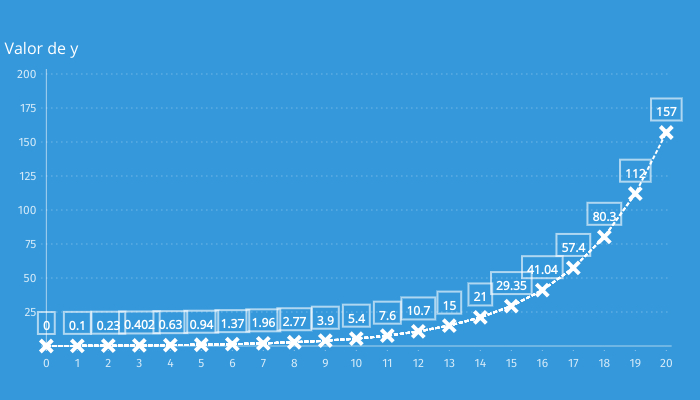
\includegraphics[width=1\textwidth]{euler.png}
\caption{\label{fig:euler}Saída dos valores aproximados com o método de euler.}
\end{figure}

\newpage
\subsection{Euler Inverso}

O método de Euler Inverso é uma variante do método de Euler, calculando o próximo valor utlizando de uma previsão a partir da próxima derivada. 
O método de euler inverso explicitado é:

\begin{equation}\label{eq:eq_euler_inverso}
    y_{n+1} = y_n + hf(t_{n+1},y_{n+1})
\end{equation}
Esta equação está na forma implícita, mas que pode ser reformulada para uma fórmula explícita, se ajustada algebricamente. Mas em com a biblioteca sympy é possível utilizar a ferramenta Solve e resolver equações diretamente sem os ajustes para uma expressão explícita.

\subsubsection{Exemplo de Entrada}
    \begin{table}[H]
        \centering
        \begin{tabular}{|c|c|c|l|l|l|}
        \hline
        Método & y0 & t0 & h   & Quantidade Passos & Função \\ \hline
        euler\_inverso  & 0  & 0  & 0.1 & 20                &  1 - t + 4y      \\ \hline
    \end{tabular}
\end{table}
\subsubsection{Método de Aproximação}
Com o auxílio da biblioteca sympy, e suas funções \textit{subs e sympify} é possível reconhecer a expressão albégrica como um objeto a ser iterado por python, e assim iterar pelos valores da função. Resolvendo a equação implícita.
\subsubsection{Exemplo de Saída}
Os valores de saída são gerados num arquivo texto. Aqui se encontram os valores em um gráfico. Na figura \ref{fig:euler_inverso}.
\begin{figure}
\centering
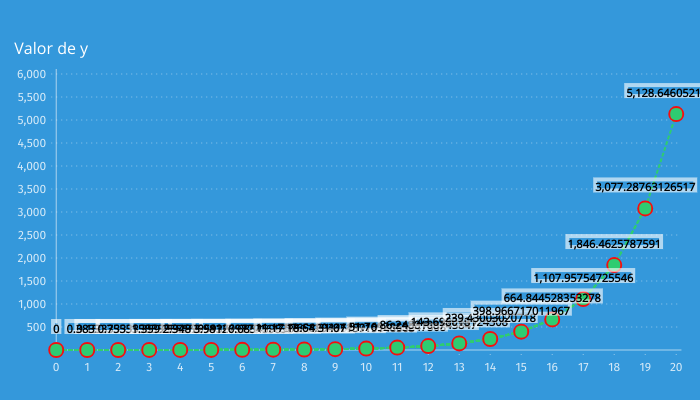
\includegraphics[width=1\textwidth]{euler_inverso.png}
\caption{\label{fig:euler_inverso}Saída dos valores aproximados com o método de Euler Inverso.}
\end{figure}


\subsection{Euler Aprimorado}

O método de Euler Aprimorado é uma variante do método de Euler, que utiliza de um ajuste do próximo passo a partir do cálculo da previsão do próximo ponto, utilizando o método de Euler. 
O método de euler Aprimorado explicitado é:

\begin{equation}\label{eq:eq_euler_aprimorado}
y_{n+1} = y_n + \frac{h(f(t_{n},y_{n}) + f(t_{n+1},y_{n+1}))}{2}
\end{equation}

\subsubsection{Exemplo de Entrada}
\begin{table}[H]
\centering
\begin{tabular}{|c|c|c|l|l|l|}
\hline
Método & y0 & t0 & h   & Quantidade Passos & Função \\ \hline
euler\_aprimorado  & 0  & 0  & 0.1 & 20                &  1 - t + 4y      \\ \hline
\end{tabular}
\end{table}
\subsubsection{Método de Aproximação}
O cálculo é feito no mesmo modelo que o Método de Euler.
\subsubsection{Exemplo de Saída}
Os valores de saída são gerados num arquivo texto. Aqui se encontram os valores em um gráfico. Na figura \ref{fig:euler_aprimorado}.
\begin{figure}
\centering
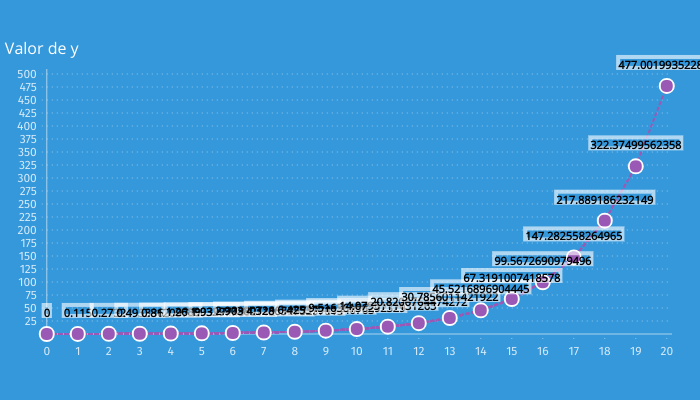
\includegraphics[width=1\textwidth]{euler_aprimorado.png}
\caption{\label{fig:euler_aprimorado}Saída dos valores aproximados com o método de Euler Aprimorado.}
\end{figure}


\newpage
\subsection{Runge Kutta}

O método de Runga Kutta estima o próximo valor a partir de uma média ponderada de alguns pontos em relação ao intervalo analisado. No caso estaremos levando em consideração o método de Runge-Kutta para o 4º grau.
O método de Runge Kutta explicitado é:


\begin{equation}\label{eq:eq_runge_kutta}
\begin{aligned}
y_{n+1} = y_n + \frac{h(k_1+2k_2+2k_3+k4)}{6} \\
k_1 = f(t_n, y_n) \\
k_2 = f(t_n + \frac{h}{2}, y_n + \frac{h}{2}k_1) \\
k_3 = f(t_n + \frac{h}{2}, y_n + \frac{h}{2}k_2) \\
k_4 = f(t_n + h, y_n + hk_3) \\
\end{aligned}
\end{equation}

\subsubsection{Exemplo de Entrada}
\begin{table}[H]
\centering
\begin{tabular}{|c|c|c|l|l|l|}
\hline
Método & y0 & t0 & h   & Quantidade Passos & Função \\ \hline
runge\_kutta  & 0  & 0  & 0.1 & 20                &  1 - t + 4y      \\ \hline
\end{tabular}
\end{table}
\subsubsection{Método de Aproximação}
O cálculo é feito no mesmo modelo que o Método de Euler.
\subsubsection{Exemplo de Saída}
Os valores de saída são gerados num arquivo texto. Aqui se encontram os valores em um gráfico. Na figura \ref{fig:runge_kutta}.
\begin{figure}
\centering
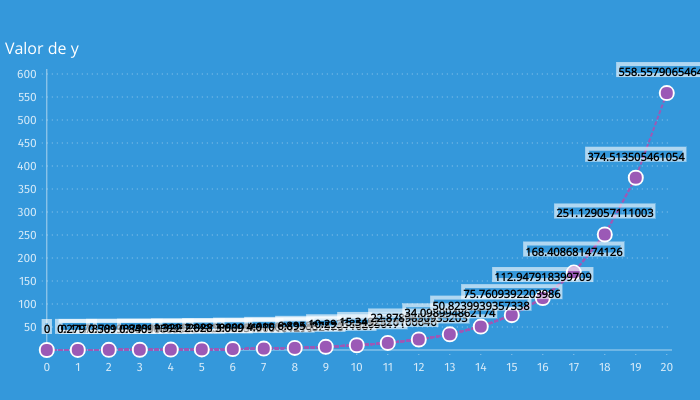
\includegraphics[width=1\textwidth]{runge-kutta.png}
\caption{\label{fig:runge_kutta}Saída dos valores aproximados com o método de Runge Kutta.}
\end{figure}


\newpage
\subsection{Adams-Bashforth}

O método de Adams-Bashforth é um método de passo múltiplos explícito que estima o próximo valor a partir do conhecimento de etapas anteriores já geradas, ao invés do método de Euler, que descarta as informações anteriores. Este método  tem vários graus, e coeficientes multiplicativos para cada um destes, analisando a tabela deste método nos requisitos do projeto, podemos escrever os métodos de Adams Bashforth no modelo:

\begin{equation}\label{eq:eq_a_b}
\begin{aligned}
Segunda Ordem: y_{n+1} = y_n + h(\beta_1f(t_{n},y_{n}) + \beta_2f(t_{n-1},y_{n-1})) \\
Terceira Ordem: y_{n+1} = y_n + h(\beta_1f(t_{n},y_{n}) + \beta_2f(t_{n-1},y_{n-1} + \beta_3f(t_{n-2},y_{n-2}))
\end{aligned}
\end{equation}
Se manter o padrão chega-se até o Adams-Bashforth de grau 8.

\subsubsection{Exemplo de Entrada}
Para o método de Adams-Bashforth existiam dois modelos de se executado: Utilizando uma lista de valores pre-estabelecidade ou utilizando um dos métodos anteriores para gerar os pontos de PVI. \par
Entrada com a lista dos elementos:
\begin{table}[H]
\centering
\begin{tabular}{|c|c|c|c|l|l|l|}
\hline
Método & y(Lista) & t0 & h   & Quantidade Passos & Função & ordem\\ \hline
adam\_bashforth  & [...]  & 0  & 0.1 & 20                &  1 - t + 4y & 5     \\ \hline
\end{tabular}
\end{table}

\begin{table}[H]
\centering
\begin{tabular}{|c|c|c|c|l|l|l|}
\hline
Método & y0) & t0 & h   & Quantidade Passos & Função & ordem\\ \hline
adam\_bashforth\_euler  & 0  & 0  & 0.1 & 20                &  1 - t + 4y & 5     \\ \hline
\end{tabular}
\end{table}


\subsubsection{Método de Aproximação}
O cálculo é feito no mesmo modelo que o Método de Euler.
\subsubsection{Exemplo de Saída}
Os valores de saída são gerados num arquivo texto. Aqui se encontram os valores em um gráfico. Na figura \ref{fig:adam_bashforth}.
\begin{figure}[H]
\centering
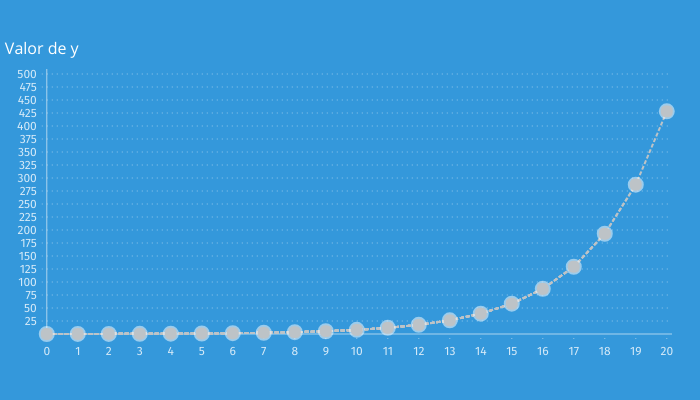
\includegraphics[width=1\textwidth]{adams.png}
\caption{\label{fig:adam_bashforth}Saída dos valores aproximados com o método de Adam Bashforth.}
\end{figure}






\subsection{Adams-Multon}

O método de Adams-Multon é um método de passo múltiplos implícito que estima o próximo valor a partir do conhecimento de etapas anteriores já geradas, ao invés do método de Euler, que descarta as informações anteriores. Este método  tem vários graus, e coeficientes multiplicativos para cada um destes, analisando a tabela deste método nos requisitos do projeto, podemos escrever os métodos de Adams Multon no modelo:

\begin{equation}\label{eq:eq_a_m}
\begin{aligned}
Segunda Ordem: y_{n+1} = y_n + h(\beta_1f(t_{n + 1},y_{n + 1}) + \beta_2f(t_{n},y_{n})) \\
Terceira Ordem: y_{n+1} = y_n + h(\beta_1f(t_{n + 1},y_{n + 1}) + \beta_2f(t_{n},y_{n} + \beta_3f(t_{n-1},y_{n-1}))
\end{aligned}
\end{equation}
Se manter o padrão chega-se até o Adams-Multon de grau 8.

\subsubsection{Exemplo de Entrada}
Para o método de Adams-Multon existiam dois modelos de se executado: Utilizando uma lista de valores pre-estabelecidade ou utilizando um dos métodos anteriores para gerar os pontos de PVI. \par
Entrada com a lista dos elementos:
\begin{table}[H]
\centering
\begin{tabular}{|c|c|c|c|l|l|l|}
\hline
Método & y(Lista) & t0 & h   & Quantidade Passos & Função & ordem\\ \hline
adam\_multon  & [...]  & 0  & 0.1 & 20                &  1 - t + 4y & 6     \\ \hline
\end{tabular}
\end{table}

\begin{table}[H]
\centering
\begin{tabular}{|c|c|c|c|l|l|l|}
\hline
Método & y0) & t0 & h   & Quantidade Passos & Função & ordem\\ \hline
adam\_multon\_euler  & 0  & 0  & 0.1 & 20                &  1 - t + 4y & 6     \\ \hline
\end{tabular}
\end{table}


\subsubsection{Método de Aproximação}
O cálculo é feito no mesmo modelo que o Método de Euler Inverso.
\subsubsection{Exemplo de Saída}
Os valores de saída são gerados num arquivo texto. Aqui se encontram os valores em um gráfico. Na figura \ref{fig:adam_multon}.
\begin{figure}[H]
\centering
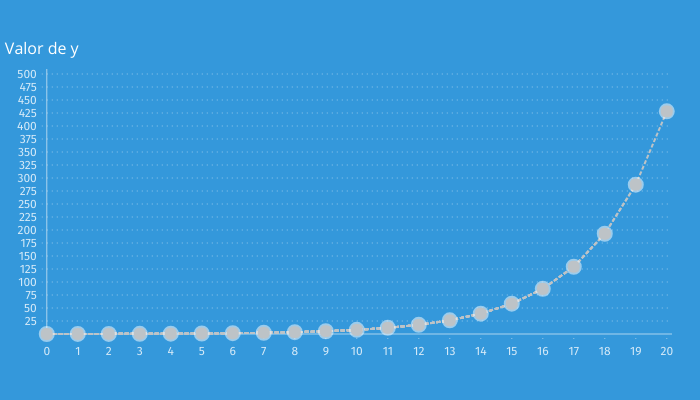
\includegraphics[width=1\textwidth]{adams.png}
\caption{\label{fig:adam_multon}Saída dos valores aproximados com o método de Adam Multon.}
\end{figure}




\newpage
\section{Análise dos Resultados}

Para analisar os resultados, se faz necessário olhar os pontos que deveriam ser gerados pela solução exata, vista na equação 4. Utilizando a mesma quantidade de passos e o intervalos. Foi gerada a curva:

\begin{figure}[H]
\centering
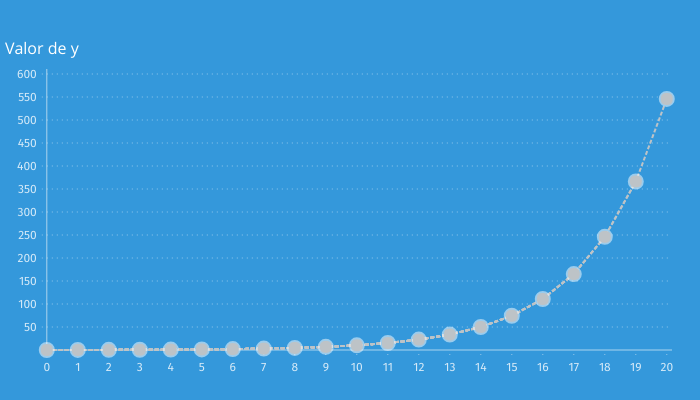
\includegraphics[width=1\textwidth]{exata.png}
\caption{\label{fig:exata}Pontos gerados pela solução exata.}
\end{figure}

\begin{figure}[H]
\centering
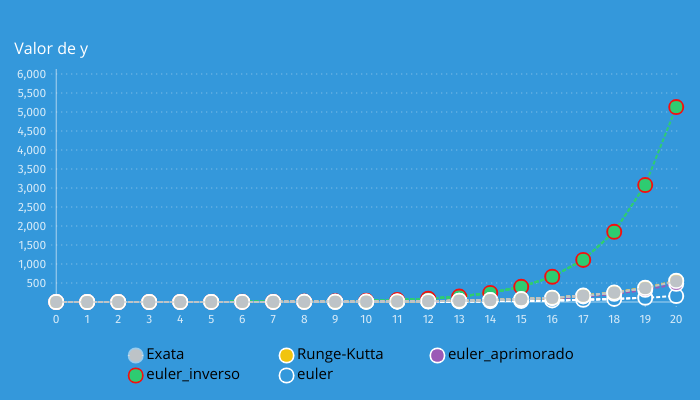
\includegraphics[width=1\textwidth]{comp_exata.png}
\caption{\label{fig:com-u}Comparação dos métodos de passos únicos e a solução exata.}
\end{figure}

\begin{figure}[H]
\centering
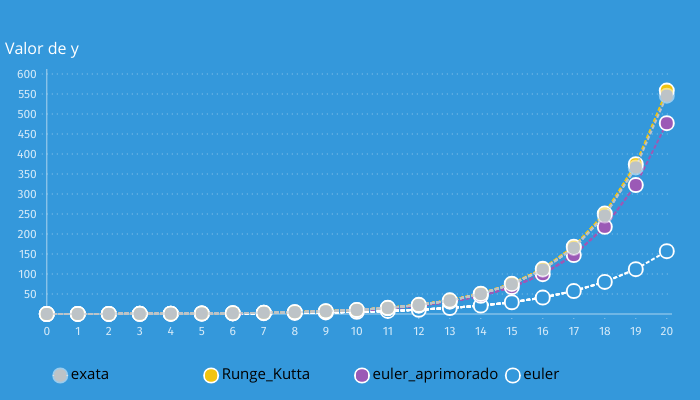
\includegraphics[width=1\textwidth]{comp_sem_inverso.png}
\caption{\label{fig:com-s-u}Comparação dos métodos de passos únicos, sem euler inverso, e a solução exata.}
\end{figure}

\begin{figure}[H]
\centering
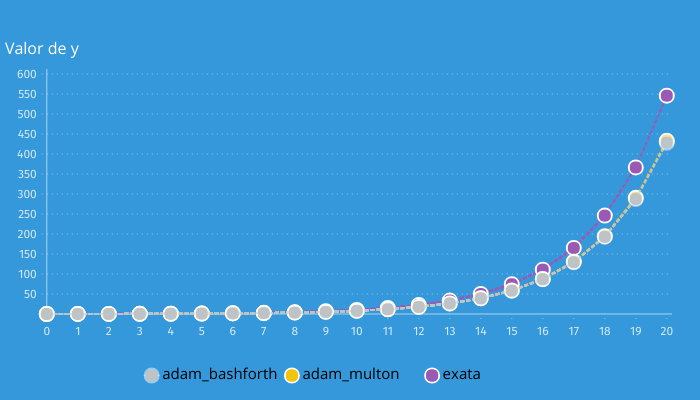
\includegraphics[width=1\textwidth]{comp_multiplos.png}
\caption{\label{fig:com-m}Comparação dos métodos de passos múltiplos e a solução exata.}
\end{figure}

Foi gerado um gráfico de comparação sem o euler inverso, para que fosse possível uma análise mais próxima entre os outros métodos, já que o euler inverso se distanciou da solução exata. \par
Dentre os métodos de passos únicos, Runge Kutta se destacou, com erros bem menores, o que era de se esperar, com uma maior quantidade de previsão e correção.
Foi perceptível que o método de adams-bashforth foi bem mais preciso do que o multon, e foi o que mais se aproximou dos resultados da solução exata.

\end{document}